\newpage

\section{Auswertung}
\subsection{Graphit}
\subsubsection{Grobe Struktur}

In Abb. \ref{fig:raw_big} ist eine Aufnahme mit der Seitenlänge 200nm (CCM-Methode) dargestellt. Man kann eine grobe Struktur unten links, sowie mehrere Kanten erkennen.

\begin{figure}[h]
    \centering
    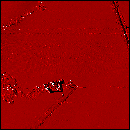
\includegraphics{data/graphit/raw_big.png}
    \caption{Graphitstruktur (Seitenlänge 200 nm)}
    \label{fig:raw_big}
\end{figure}

\subsubsection{Atomare Auflösung}
Unsere Spitze war geeignet, atomare Auflösung bei Graphit zu erreichen. In Abb. \ref{fig:raw} ist das gemessene Bild (CHM-Methode) dargestellt. Da das Bild stark verrauscht ist, wurde ein Fourierfilter angewendet. Das Ergebnis ist in Abb. \ref{fig:edit} dargestellt. Man kann gut das sechseckige Gitter, dass die weißen Bereiche aufspannen, erkennen. Das sind die Punkte, in denen zwei Kohlenstoffatome übereinander liegen. Es handelt sich also nicht um die sechseckige Graphitstruktur, sondern nur um einen Teil davon. Für die Auswertung der Winkel können diese Punkte aber trotzdem verwendet werden, da die Winkel der Gitterstruktur gleich den Winkeln der Sechsecke sind.\\

\begin{figure}[h]
  \centering
  \begin{subfigure}[h]{0.5\textwidth}
    \centering
    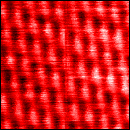
\includegraphics{data/graphit/raw.png}
    \subcaption{Seitenlänge 200 nm}
    \label{fig:raw}
  \end{subfigure}%
  \begin{subfigure}[h]{0.5\textwidth}
    \centering
    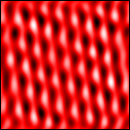
\includegraphics{data/graphit/2nm_edit2.png}
    \subcaption{Mit Fourierfilter überarbeitet, Seitenlänge 2 nm}
    \label{fig:edit}
  \end{subfigure}
  \caption{Graphitstruktur mit atomarer Auflösung}
\end{figure}

\begin{figure}
\centering
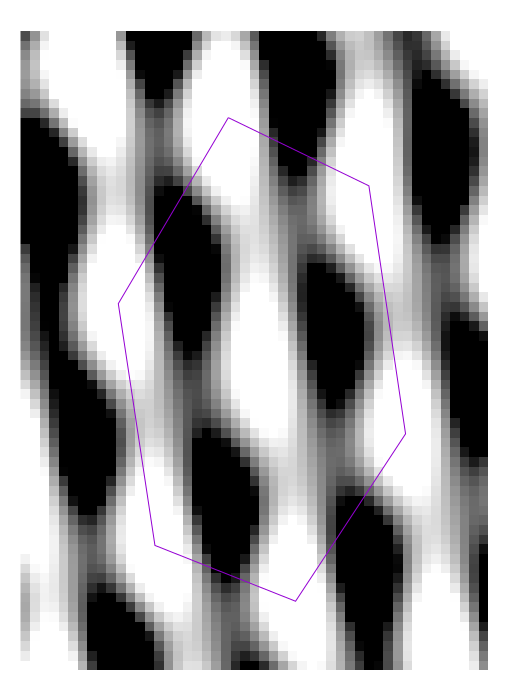
\includegraphics[scale=0.35]{data/graphit/graphit.png}
\caption{Ausschnitt mit ermittelten Mittelpunkten}
\label{fig:small}
\end{figure}

In einem kleinen Ausschnitt (siehe Abb. \ref{fig:small}) wird nun ein solches Sechseck vermessen. Die Mittelpunkte der weißen Bereiche relativ zum weißen Bereich in der Mitte sind in Tab.\ref{tab:points} dargestellt (Fehler $\Delta x=\Delta y=$ 0,01 nm).

\newpage

\begin{table}
\centering
\begin{tabular}{ccc}
\toprule
n & x/nm & y/nm\\
\midrule
1 & -0,05 &-0,41\\
2 & 0,18&	-0,3\\
3 & 0,24&	0,1\\
4 & 0,06&	0,37\\
5 & -0,17&	0,28\\
6 & -0,23&	-0,11\\
\bottomrule
\end{tabular}
\caption{Bestimmte Mittelpunkte der weißen Bereiche}
\label{tab:points}
\end{table}
 
Die Punkte bilden offensichtlich kein regelmäßiges Sechseck. Das liegt daran, dass das Bild verzerrt wurde. Um es zu entzerren, drehen wir erst das Bild um den Winkel $\phi$, so dass die Verzerrungsachse in Richtung y-Achse zeigt. Dann verzerren wir das Bild in Richtung y-Achse um den Faktor $\alpha$. Die einzelnen Punkte sollten dann möglichst auf einem Kreis mit Radius $r$ liegen. Dazu sollte der Abstand aller Punkte zum Ursprung etwa $r$ sein.\\

Um ein möglichst gutes Ergebnis zu erhalten, machen wir eine Anpassung über die freien Parameter $\phi, \alpha, r$, um die folgende Funktion zu minimieren:
\begin{align*}
f(\phi,\alpha,r) &= \sum\limits_{n = 1}^6 \left(\left|
\begin{pmatrix}
1 & 0\\
0 & \alpha
\end{pmatrix}
\begin{pmatrix}
\cos{\phi} & \sin{\phi}\\
-\sin{\phi} & \cos{\phi}
\end{pmatrix}
\begin{pmatrix}
x_n\\
y_n
\end{pmatrix}
  \right| - r\right)^2
\end{align*}.
Die rechte Matrix dreht das Polygon und die linke verzerrt die y-Achse. Danach wird von der Norm des Vektors $r$ abgezogen und das Quadrat dieser Abweichung aufsummiert. Somit soll sichergestellt werden, dass alle Punkte am Ende näherungsweise auf einem Kreis liegen. Dabei muss beachtet werden, dass das Original in einer Richtung gestaucht wurde. Somit muss $\alpha > 1$ gelten (um die Stauchung rückgängig zu machen).\\
Die Anpassung (siehe Tab.\ref{tab:fit}, Abb. \ref{fig:fit1}, Abb. \ref{fig:fit2}) ergibt: $\phi = 91,7^\circ \pm 2^\circ$, $\alpha = 1,64 \pm 0,06$, $r = (0,403 \pm 0,008)\si{\nano\metre}$. Die Fehler erhält man dabei aus den Fehlern für die Positionen, indem man die impliziten Funktionen ($\phi(\vec{x},\vec{y})$ etc.) numerisch differenziert.  \\ 

Wie man in Abb. \ref{fig:fit2} erkennt, liegen die Punkte jetzt fast auf einem Kreis, sie sind nur etwas verschoben. In Tab. \ref{tab:res} sind die gemessenen Kantenlängen und Innenwinkel aufgetragen. Durch Mittelung (Fehler über Standartabweichung) ergibt sich $l = (0,410 \pm 0,004)$ nm und $\varphi = 120^\circ \pm 3^\circ$. Dass der Wert für $\varphi = 120^\circ$ beträgt, liegt nicht an einer genauen Messung, sondern daran, dass jedes Sechseck eine Innenwinkelsumme von $720^\circ$ hat. Demzufolge ist nur der Fehler ausschlaggebend. Bei $\Delta\varphi=3^\circ$ kann man davon ausgehen, dass es sich um gleichseitige Sechsecke handelt und somit Graphit eine Gitterstruktur aus regelmäßigen Sechsecken hat. Es ist zu beachten, dass die berechneten Längen aufgrund der Verzerrung nicht den tatsächlichen Abständen entsprechen müssen, sondern lediglich zeigen sollen, dass das Gitter bei senkrechter Betrachtung die erwartete Struktur aufweist.

\begin{figure}[h]
  \centering
  \begin{subfigure}{0.5\textwidth}
    \centering
    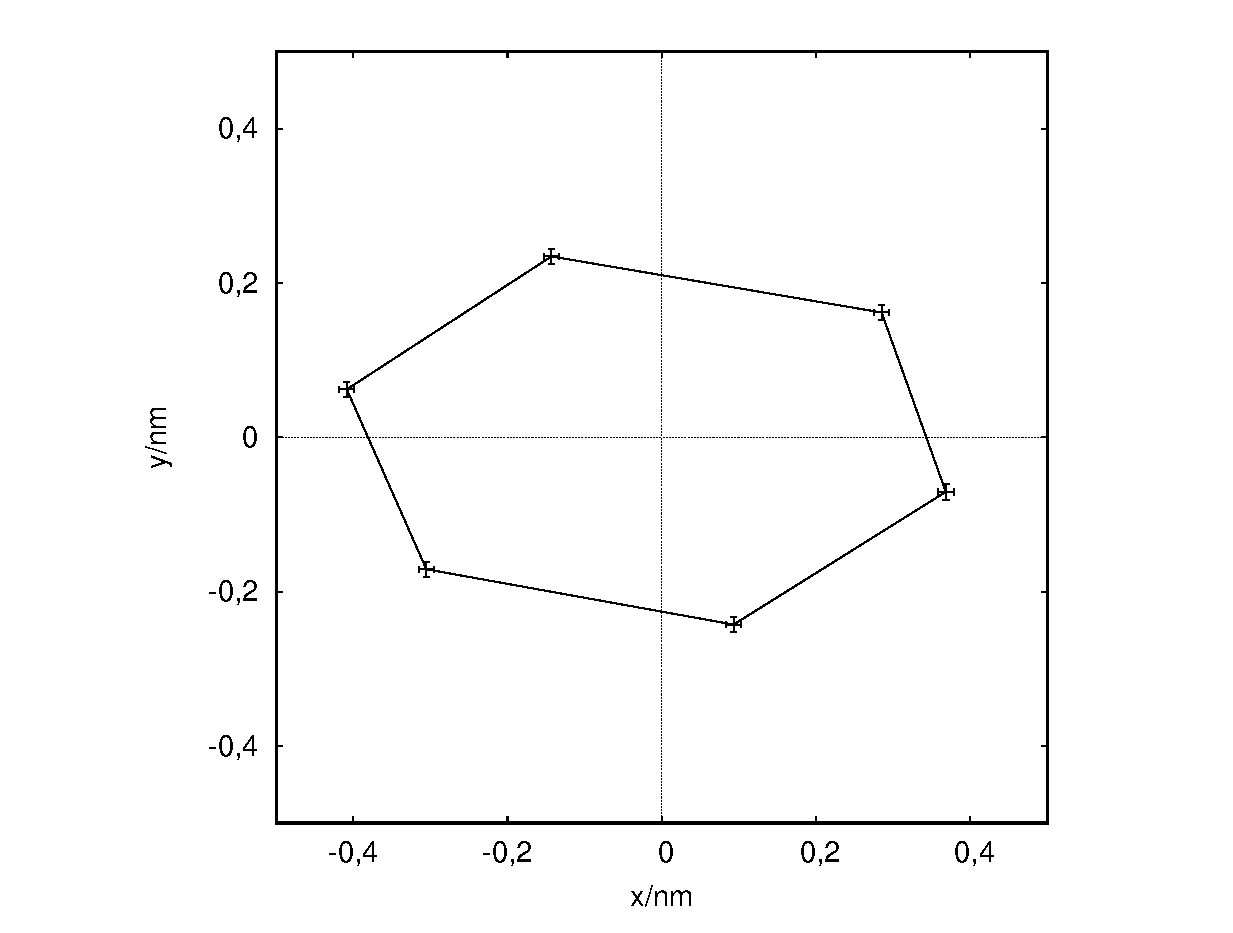
\includegraphics[width=1\textwidth]{data/graphit_kilian/out_rotate_old.eps}
    \subcaption{Nach Drehung um Winkel $\phi=91,7^\circ$}
    \label{fig:fit1}
  \end{subfigure}%
  \begin{subfigure}{0.5\textwidth}
    \centering
    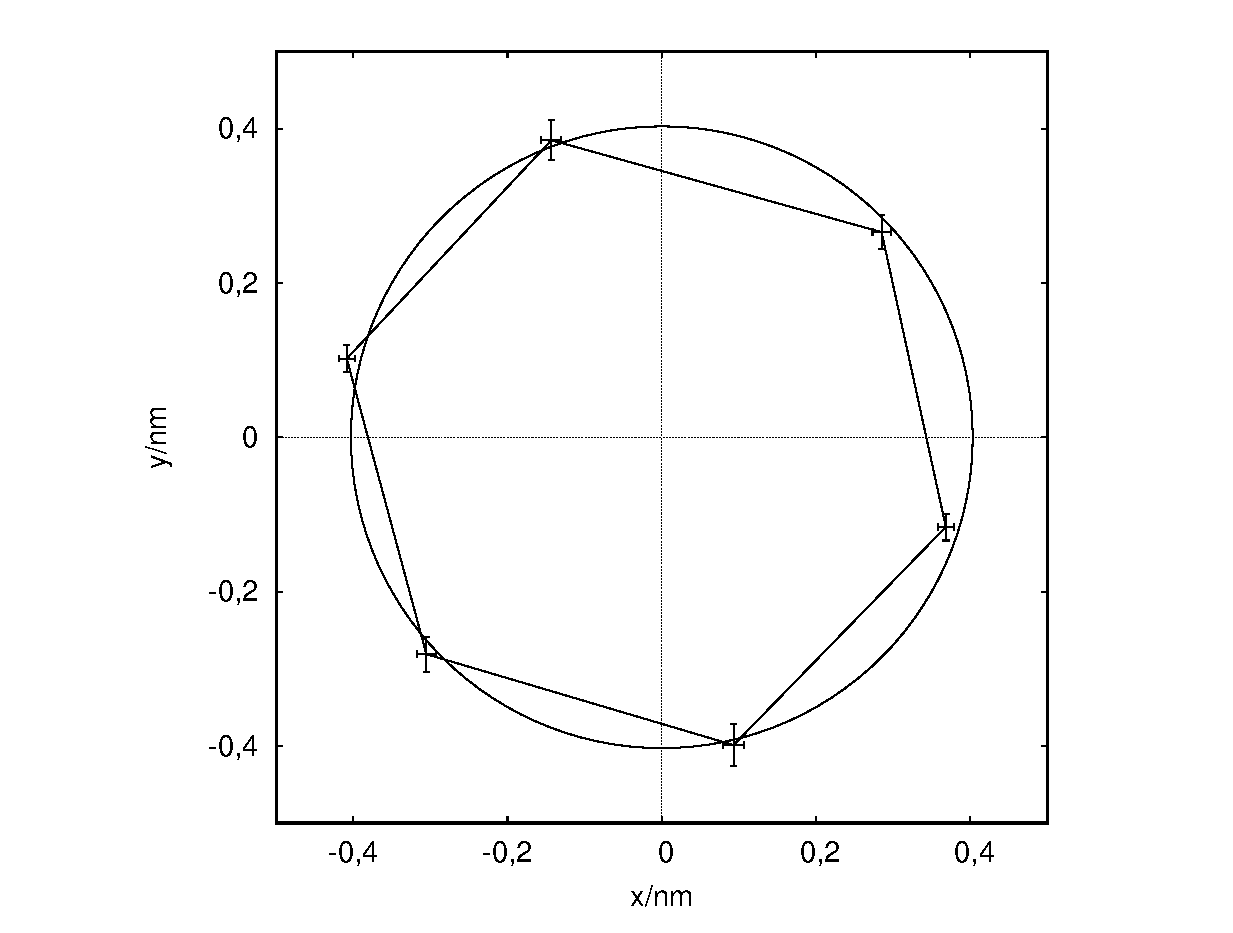
\includegraphics[width=1\textwidth]{data/graphit_kilian/out_rotate.eps}
    \subcaption{Nach Drehung und Entzerrung}
    \label{fig:fit2}
  \end{subfigure}
  \caption{Geometrische Transformation von Gitter}
\end{figure}

\begin{table}[h]
  \centering
  \begin{subtable}[h]{0.5\textwidth}
    \centering
    \begin{tabular}{ccc}
      \toprule
      n & x/nm & y/nm\\
      \midrule
      1&	-0,41&	0,101\\
      2&	-0,31&	-0,28\\
      3& 0,09&	-0,40\\
      4&	0,36&	-0,12\\
      5&	0,28&	0,27\\
      6&	-0,10&	0,38\\
      \bottomrule
    \end{tabular}
    \subcaption{Koordinaten, $\Delta x=$0,01 nm, $\Delta y=$0,03 nm }
    \label{tab:fit}
  \end{subtable}%
  \begin{subtable}[h]{0.5\textwidth}
    \centering
    \begin{tabular}{>{$}c<{$}cc}
      \toprule
      n & l/nm & $\varphi/^\circ$\\
      \midrule
      1 \to 2 & 0,39$\pm$0,04 & 118$\pm$7\\
      2 \to 3 & 0,415$\pm$0,006 & 122$\pm$7\\
      3 \to 4 & 0,39$\pm$0,04 & 118$\pm$7\\
      4 \to 5 & 0,39$\pm$0,04 & 123$\pm$8\\
      5 \to 6 & 0,405$\pm$0,006 & 119$\pm$7\\
      6 \to 1 & 0,41$\pm$0,04 & 121$\pm$7\\
      \bottomrule
    \end{tabular}
    \subcaption{Abstände und Innenwinkel}
    \label{tab:res}
  \end{subtable}
  \caption{Gittergrößen nach Entzerrung}
\end{table}

Um die Atomabstände $a$ von Graphit zu bestimmen, werden mehrere Sechsecke in Abbildung \ref{fig:edit} vermessen. Das Ergebnis ist in Abbildung \ref{fig:measurement} zu sehen. Die mit \textit{ImageJ} gemessenen Abstände sind in Tabelle \ref{tab:measurement} zu finden. Für die gemessenen Strecken wird ein Fehler von $\Delta l=0,02$ nm angenommen. Der mittlere gemessene Abstand entspricht somit $l=(0,311 \pm 0,004)$ nm. 
Nun muss beachtet werden, dass die weißen Punkte nur die Atome darstellen, die direkt über einem anderen sind. Drei benachbarte Atome in einem Sechseck bilden ein gleichschenkliges Dreieck mit der Basis $l$ und den Atomabständen $a$ als Schenkel (siehe Abb. \ref{fig:triangle}). Der Winkel an der Spitze beträgt $120^\circ$. Damit ergibt sich
\begin{align*}
a\cdot\sin{\frac{120^\circ}{2}} &= \frac{l}{2}\\
\rightarrow a &= \frac{l}{\sqrt{3}}\\
  &= (0,179 \pm 0,002) \ \mathrm{nm}.
\end{align*} Der berechnete Abstand der Atome beträgt also $a = (0,179 \pm 0,002) \ \si{\nano\metre}$. Der Literaturwert liegt bei $l=0,142$ nm (siehe \cite{graphit}). Diese Abweichung ist für das Betrachten einer verkippten Aufnahme nicht verwunderlich. Trotzdem konnte die atomare Gitterstruktur von Graphit eindeutig bestätigt werden.

\begin{figure}[h]
  \centering
  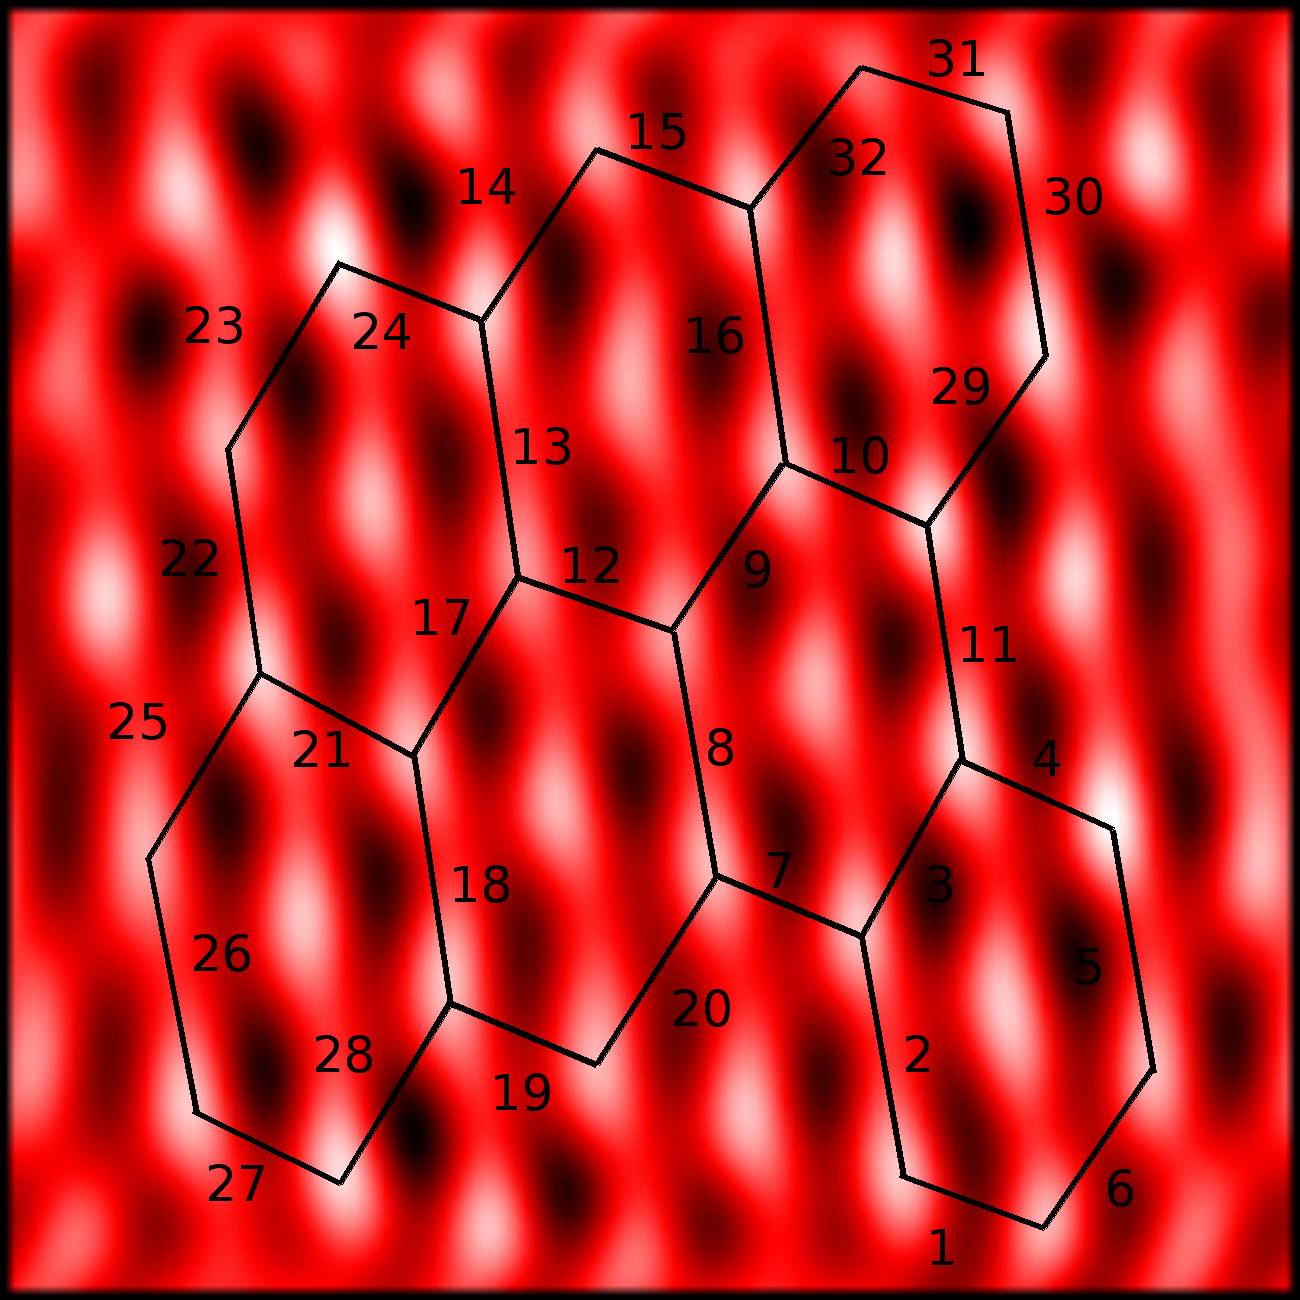
\includegraphics[width=0.5\textwidth]{data/graphit_kilian/measurement_final.png}
  \caption{gemessene Abstände in Graphitstruktur}
  \label{fig:measurement}
\end{figure}

\begin{figure}[h]
\centering
\definecolor{qqwuqq}{rgb}{0.,0.39215686274509803,0.}
\definecolor{ffffff}{rgb}{1.,1.,1.}
\begin{tikzpicture}[line cap=round,line join=round,>=triangle 45,x=3.0cm,y=3.0cm]
\clip(-1.798235627638573,-1.1694768704984821) rectangle (2.968878775383718,1.243097549118033);
\draw [shift={(0.,0.)},color=qqwuqq,fill=qqwuqq,fill opacity=0.10000000149011612] (0,0) -- (-60.:0.12435950616579888) arc (-60.:0.:0.12435950616579888) -- cycle;
\draw (-0.5,0.8660254037844388)-- (0.5,0.8660254037844386);
\draw (0.5,0.8660254037844386)-- (1.,0.);
\draw (1.,0.)-- (0.5,-0.866025403784439);
\draw (0.5,-0.866025403784439)-- (-0.5,-0.8660254037844384);
\draw (-0.5,-0.8660254037844384)-- (-1.,0.);
\draw (-1.,0.)-- (-0.5,0.8660254037844388);
\draw [dash pattern=on 1pt off 1pt] (0.5,0.8660254037844386)-- (1.5,0.866025403784439);
\draw [dash pattern=on 1pt off 1pt] (0.5,0.8660254037844386)-- (0.,0.);
\draw [dash pattern=on 1pt off 1pt] (0.,0.)-- (0.5,-0.866025403784439);
\draw [dash pattern=on 1pt off 1pt] (0.5,-0.866025403784439)-- (1.5,-0.8660254037844395);
\draw [dash pattern=on 1pt off 1pt] (1.5,-0.8660254037844395)-- (2.,0.);
\draw [dash pattern=on 1pt off 1pt] (1.5,0.866025403784439)-- (2.,0.);
\draw [dotted] (0.5,0.8660254037844385)-- (0.5,-0.8660254037844392);
\draw [dotted] (0.,0.)-- (0.5,0.);
\begin{scriptsize}
\draw [fill=ffffff] (0.,0.) circle (2.5pt);
\draw[color=black] (0.2039524216307892,0.5031584874315245) node {a};
\draw[color=black] (0.2039524216307892,-0.4295378088119736) node {a};
\draw [fill=ffffff] (0.5,0.8660254037844385) circle (2.5pt);
\draw[color=ffffff] (0.5272871376618663,0.9425620758840169) node {$E$};
\draw [fill=ffffff] (0.5,-0.8660254037844392) circle (2.5pt);
\draw[color=ffffff] (0.5272871376618663,-0.790180376692793) node {$F$};
\draw [fill=ffffff] (-1.,0.) circle (2.5pt);
\draw[color=ffffff] (-0.9691722531999137,0.07619084959561201) node {$G$};
\draw [fill=ffffff] (2.,0.) circle (2.5pt);
\draw[color=ffffff] (2.02789184539584,0.07619084959561201) node {$H$};
\draw[color=black] (0.5314324545340595,-0.031587389081414445) node {l};
\draw [fill=ffffff] (1.,0.) circle (2.5pt);
\draw[color=ffffff] (1.041306429813835,0.07619084959561201) node {$F'$};
\draw[color=qqwuqq] (0.08788354920937688,-0.019151438464834462) node {60\textrm{\degre}};
\end{scriptsize}
\end{tikzpicture}
\caption{Zwei Sechsecke in unterschiedlichen Ebenen}
\label{fig:triangle}
\end{figure}


\subsection{Gold}
In Abb. \ref{fig:gold} ist eine Aufnahme mit der Seitenlänge 100 nm (CCM-Methode) dargestellt.  Da der linke Teil deutlich heller ist, ist er höher als der rechte. Wir denken also, dass die Aufnahme an einer Kante entstanden ist. Im Vergleich zu Graphit wirkt die Aufnahme verschwommen und es bilden sich wolkenartige Strukturen. Dies liegt daran, dass die Ladungsdichte in Gold deutlich homogener verteilt ist als in Graphit. Demzufolge war es uns auch nicht möglich eine Aufnahme mit atomarer Auflösung herzustellen. Um die atomare Oberfläche von Gold zu betrachten, bräuchte man eine andere Methode wie z.B. ein Rasterkraftmikroskop.

\begin{figure}[h]
\centering
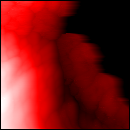
\includegraphics[scale=1]{data/gold/raw.png}
\caption{Grobe Goldstruktur (Seitenlänge 100 nm)}
\label{fig:gold}
\end{figure}

\subsection{TaS$_2$}
In Abb. \ref{fig:tas2} ist eine Aufnahme mit der Seitenlänge 84,7 nm (CCM-Methode) dargestellt. Auch hier kann man grobe Strukturen erkennen, die höher liegen als andere. Eine Abbildung mit atomarer Auflösung aufzunehmen war leider nicht möglich. Demzufolge konnten wir auch keine Ladungsdichtewellen erkennen. 

\begin{figure}[h]
\centering
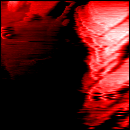
\includegraphics[scale=1]{data/tas2.png}
\caption{Grobe TaS$_2$-Struktur (Seitenlänge 84,7 nm)}
\label{fig:tas2}
\end{figure}
